\documentclass[a4paper]{article}

\usepackage{amsthm}

\newcommand{\any}{{*}}

\usepackage{tikz}

\newtheorem{theorem}{Theorem}[section]
\newtheorem{lemma}[theorem]{Lemma}
\newtheorem{proposition}[theorem]{Proposition}


\title{Coloring de Bruijn graphs}

\author{Johannes Marti and Leif Sabellek}

\begin{document}

\maketitle

\section{Notation}

If a length $k$ is obvious from the context we write $w\dots$ for $w \in
\{0,1\}^+$ for the word $w w w w w w w w w w w w \dots$ truncated to
length $k$. Usually, the length of $w$ will be smaller than $k$.

We write $s \rightarrow_i t$ for $i \in \{0,1\}$ if in the pattern there
is an $i$-edge from $s$ to $t$.

We assume that the pattern is such that every node has either just
outgoing $0$-edges or just outgoing $1$-edges. Then call a node a
$i$-node if it has just outgoing $i$-edges. A pattern is a $n$-$m$
pattern if it has at most $n$ many $0$-nodes and at most $m$ many
$1$-nodes. 

We also call a homomorphism $h$ from $T_n$ to $P$ for some $n$ and $X$
pattern $P$ a \emph{$X$ coloring} of $T_n$. The vertices of the pattern
$P$ are also called \emph{colors}. A $\hat{n}$-$m$ coloring $h$ is a
$n$-$m$ coloring such that $h(0\dots) \rightarrow_0 c$ for all $0$-nodes
$c$ in the image of $h$. Similarly, a $\hat{n}$-$\hat{m}$ coloring $h$
is a $n$-$m$ coloring such that $h(0\dots) \rightarrow_0 c$ and
$h(1\dots) \rightarrow_1 d$ for all $0$-nodes $c$ and $1$-nodes $d$ in
the image of $h$.

\section{$n$-$1$ colors}

\begin{lemma} \label{l:path to other loop}
 If $h$ is a $n$-$1$ coloring of $T_k$ then there are colors
$a_1,\dots,a_{n - 1}$ such that there is a path
\[
 h(0\dots) \rightarrow_0 a_1 \rightarrow_0 \dots \rightarrow_0 a_{n - 1}
\rightarrow_0 h(1\dots).
\]
\end{lemma}
\begin{proof}
 There is a $0$ path of length $k$ from $h(0\dots)$ to $h(1\dots)$ in
$T_k$. If $k > n$ then at least one $0$ node occurs twice on this path.
Thus we can shorten the path until we obtain a $0$ path of length $l$
with $l \leq n$ from $h(0\dots)$ to $h(1\dots)$. If $l = n$ then we have
already proven the statement of the lemma. If $l < n$ then we can extend
the path to one of length $n$ by just repeating the $0$ loop at
$h(0\dots)$ in the beginning of the path.
\end{proof}

\begin{lemma} \label{l:loop sees all}
 If $h$ is a $n$-$1$ coloring of $T_k$ then $h(1\dots) \rightarrow_1 a$
for every $0$ node $a$ in the image of $h$.
\end{lemma}
\begin{proof}
 Note that in the de Bruijn graph every node has a $1$ predecessor.
Because in the pattern there is only one $1$ node $h(1\dots)$ it follows
that all of these predecessors are mapped to $h(1\dots)$. Because $h$ is
a homomorphism it follows that $h(1\dots)$ is the $1$ predecessor of
every node in the image of $h$.
\end{proof}

\begin{proposition}[$T_n$ suffices for $n$-$1$ patterns]
 Let $h$ be an $n$-$1$ coloring of $T_k$ for some $k$. Then
there is a homomorphism $g$ from $T_n$ to $P$.
\end{proposition}
\begin{proof}
Let $P$ be the pattern in the coloring $h$ and define the the
homomorphism $g$ from $T_n$ to $P$ such that:
\[
 \begin{array}{rcl}
 0\dots0 & \mapsto & h(0\dots) \\
 0\dots01 & \mapsto & a_1 \\
 0\dots01x & \mapsto & a_2 \\
 \vdots & \mapsto & \vdots \\
 0\dots01x_1\dots x_j & \mapsto & a_{j + 1} \\
 \vdots & \mapsto & \vdots \\
 01x_1\dots x_{n - 2} & \mapsto & a_{n - 1} \\
 \end{array} \quad
 \begin{array}{rcl}
 1x_1\dots x_{n - 1} & \mapsto & h(1\dots) \\
 \end{array}
\]
Here, $a_1,\dots,a_{n - 1}$ are as in Lemma~\ref{l:path to other loop}.
To check that this is a homomorphism we use Lemmas \ref{l:path to
other loop}~and~\ref{l:loop sees all}.
\end{proof}

\section{$2$-$2$ colors}

The following is a $2$-$2$ pattern that colors $T_3$ but not $T_2$:
\begin{center}
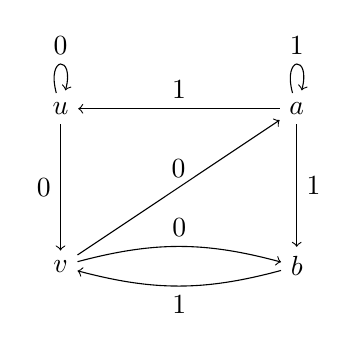
\begin{tikzpicture}
 \node (u) at (0,2) {$u$};
 \node (v) at (0,0)  {$v$};

 \node (a) at (3,2) {$a$};
 \node (b) at (3,0)  {$b$};

 \draw [->] (u) edge node[left] {$0$} (v);
 \draw [->] (u) edge [loop above] node[above] {$0$} (u);

 \draw [->] (a) edge node[right] {$1$} (b);
 \draw [->] (a) edge [loop above] node[above] {$1$} (a);

 \draw [->] (v) edge node[above] {$0$} (a);
 \draw [->] (v) edge [bend left=15] node[above] {$0$} (b);

 \draw [->] (a) edge node[above] {$1$} (u);
 \draw [->] (b) edge [bend left=15] node[below] {$1$} (v);
\end{tikzpicture}
\end{center}

Our goal is to show that $T_3$ colors all colorable $2$-$2$ patterns. We
start with two lemmas.

The first lemma shows that every $2$-$2$ coloring is already a
$\hat{2}$-$\hat{2}$ coloring.
\begin{lemma} \label{reachability lemma}
 If there is a homomorphism $h$ from $T_k$ to a $2$-$2$ pattern $P$ then
$h(0\dots) \rightarrow_0 s$ for all $0$-node $s$ in the image of $h$.
\end{lemma}
\begin{proof}
 First observe that $h(0\dots) \rightarrow_0 h(0\dots)$, because $h$ is
a homomorphism. Note that there is at most one $0$-node $s$ that is
distinct from $h(0\dots)$ because there are at most two $0$-nodes in
$P$. Assume that $s \neq h(0\dots)$ is in the image of $h$, that is, $s
= h(x)$ for some $x$ in $T_k$. We show that then $h(0\dots)
\rightarrow_0 s$. Because there is a $0$-path from $0\dots$ to $x$ in
$T_k$ there must also be a $0$-path from $h(0\dots)$ to $s$. All nodes
on this path are $0$-nodes and thus they are either equal to $h(0\dots)$
or to $s$ since $P$ does contain no more than two $0$-nodes. Consider
the first occurrence of $s$ on this path. It is not possible that this is
the start node of the path because $h(0\dots) \neq s$. But then the
predecessor of the first occurrence of $s$ must be $h(0\dots)$ and hence
$h(0\dots) \rightarrow_0 s$.
\end{proof}

\begin{lemma} \label{between lemma}
 If there is a homomorphism $h$ from $T_k$ to a $2$-$2$ pattern $P$ then
there is a $0$-node $s$ in $P$ such that $h(10\dots) \rightarrow_1
s \rightarrow_0 h(1\dots)$.
\end{lemma}
\begin{proof}
Consider a path $v_0 \rightarrow_1 v_1 \rightarrow_0
v_2 \rightarrow_1 \dots \rightarrow_0 v_l$ in $p$ from $v_0 =
h(10\dots)$ to $v_l = h(1\dots)$. This path must exists because it is
easy to see that an alternating $0$ and $1$ path from $10\dots$ to
$1\dots$ exists in $T_k$. note that $l$ is even because the path is
alternating. In fact one could argue more carefully that its length must
be largest even number smaller or equal to $k$.

We can proof the claim with in induction on the length of this path. If
the length of the path is $0$ then $h(10\dots) = h(1\dots)$ and thus we
can set $s = h(01\dots)$ because $h(10\dots) \rightarrow_1 h(01\dots)$
and $h(01\dots) \rightarrow_0 h(10\dots)$.

If the length $l$ of the path is larger than $0$ then it can be split
into a path $v_0 \rightarrow_1 \dots \rightarrow_0 v_{l - 2}$ and a
length $2$ path $v_{l - 2} \rightarrow_1 v_{l - 1} \rightarrow_0 v_l$.
Because $P$ contains at most two $1$-vertices we have either that
$h(10\dots) = h(1\dots)$, or that $v_{l - 2} = h(10\dots)$, or that
$v_{l - 2} = h(1\dots)$.

In the first case where $h(10\dots) = h(1\dots)$ we have already seen that we
can set $s = h(01\dots)$.

In the case where $v_{l - 2} = h(10\dots)$ we can set $s = v_{l - 1}$
because $v_{l - 2} \rightarrow_1 v_{l - 1} \rightarrow_0 v_l$ and $v_l =
h(1,\dots)$.

In the last case where $v_{l - 2} = h(1\dots)$, we can simply apply the
induction hypothesis to the path $v_0 \rightarrow_1 \dots \rightarrow_0
v_{l - 2}$.
\end{proof}

\begin{proposition}[$T_3$ suffices for $2$-$2$ colors]
 Let $P$ be a $2$-$2$ pattern such that there is a homomorphism $h$ from
$T_k$, for some $k > 3$, to $P$. Then there is a homomorphism $g$ from
$T_3$ to $P$.
\end{proposition}
\begin{proof}
Define $g$ from $T_3$ to $P$ such that it maps as follows
\[
 \begin{array}{rcl}
 000 & \mapsto & h(0\dots) \\
 001 & \mapsto & h(0\dots) \\
 010 & \mapsto & h(01\dots) \\
 011 & \mapsto & s_0
 \end{array} \quad
 \begin{array}{rcl}
 111 & \mapsto & h(1\dots) \\
 110 & \mapsto & h(1\dots) \\
 101 & \mapsto & h(10\dots) \\
 100 & \mapsto & s_1
 \end{array}
\]
Here, $s_0$ is the node which exists by Lemma~\ref{between lemma} and
$s_1$ is the analogous node which exists by swapping all $0$s and $1$s
in the lemma. It is left to the reader to check that this defines a
homomorphism. At most edges this follows because $h$ is a homomorphism,
and for the more difficult edges one uses Lemmas \ref{reachability
lemma}~and~\ref{between lemma}.
\end{proof}

\section{$\hat{n}$-$2$ colorings}

\begin{lemma} \label{hat one}
 If $h$ is a $n$-$2$ coloring of $T_k$ then there are colors $a$
and $u$ in the image of $h$ such that
\[
 h(10\dots) \rightarrow_1 a \rightarrow_0 u \rightarrow_1 h(0\dots).
\]
\end{lemma}
\begin{proof}
 Note first that there is an alternating $10 \dots$ path in $T_k$ from
$10\dots$ to $0 \dots$. This path has an odd length. Because $h$ is a
homomorphism the path then also exists in the image of $h$ where it
starts at $h(01\dots)$ and stops at $h(0\dots)$. Now if the path is
longer than $3$ then we can shorten it: In this case it passes over more
than two $1$ nodes and hence at least one $1$ color occurs twice in the
path. If the path shortens to one of length $3$ we are done. If it
shortens to a path of length $1$ then it is of the form $h(10\dots)
\rightarrow_1 h(0\dots)$. We can still get the required path of length
$3$ by setting $a = h(01\dots)$ and $u = h(10\dots)$.
\end{proof}

\begin{lemma} \label{hat two}
 If $h$ is a $n$-$2$ coloring of $T_k$ then there are colors $v$
and $b$ in the image of $h$ such that
\[
 h(01\dots) \rightarrow_0 v \rightarrow_1 b \rightarrow_0 h(1\dots).
\]
\end{lemma}
\begin{proof}
 Note first that there is an alternating $01 \dots$ path in $T_k$ from
$01\dots$ to $1 \dots$. This path has an odd length. Because $h$ is a
homomorphism the path then also exists in the image of $h$ where it
starts at $h(10\dots)$ and stops at $h(1\dots)$. Now if the path is
longer than $3$ then we can shorten it: In this case it passes over more
than two $1$ nodes and hence at least one $1$ color occurs twice in the
path. If the path shortens to one of length $3$ we are done. If it
shortens to a path of length $1$ then it is of the form $h(01\dots)
\rightarrow_0 h(1\dots)$. We can still get the required path of length
$3$ by setting $v = h(10\dots)$ and $b = h(01\dots)$.
\end{proof}

\begin{proposition}[$T_4$ suffices for $\hat{n}$-$2$ colorings]
 Let $h$ be an $\hat{n}$-$2$ coloring of $T_k$ for some $k > 4$. Then
there is a homomorphism $g$ from $T_4$ to $P$.
\end{proposition}
\begin{proof}
Let $P$ be the pattern in the coloring $h$ and define the the
homomorphism $g$ from $T_4$ to $P$ such that:
\[
 \begin{array}{rcl}
 00\any\any & \mapsto & h(0\dots) \\
 0100 & \mapsto & a \\
 0101 & \mapsto & h(01\dots) \\
 011\any & \mapsto & b
 \end{array} \quad
 \begin{array}{rcl}
 11\any\any & \mapsto & h(1\dots) \\
 1011 & \mapsto & v \\
 1010 & \mapsto & h(10\dots) \\
 100\any & \mapsto & u
 \end{array}
\]
Here, $a$ and $u$ are as in the statement of Lemma~\ref{hat one} and $v$
and $b$ are as in the statement of Lemma~\ref{hat two}. It is left to
the reader to check that this defines a homomorphism.
\end{proof}


\section{$\hat{n}$-$\hat{3}$ colorings}

As in the previous section we can prove the following lemmas:
\begin{lemma} \label{three zero}
 If $h$ is a $n$-$3$ coloring of $T_k$ then there are colors $a_1$,
$u_2$, $a_3$ and $u_4$ in the image of $h$ such that
\[
 h(10\dots) \rightarrow_1 a_1 \rightarrow_0 u_2 \rightarrow_1 a_3
\rightarrow_0 u_4 \rightarrow_1 h(0\dots).
\]
\end{lemma}

\begin{lemma} \label{three one}
 If $h$ is a $n$-$3$ coloring of $T_k$ then there are colors $u_1$,
$a_2$, $u_3$ and $a_4$ in the image of $h$ such that
\[
 h(01\dots) \rightarrow_0 u_1 \rightarrow_1 a_2 \rightarrow_0 u_3
\rightarrow_1 a_4 \rightarrow_0 h(1\dots).
\]
\end{lemma}

We then obtain:
\begin{proposition}[$T_6$ suffices for $\hat{n}$-$\hat{3}$ colorings]
 Let $h$ be an $\hat{n}$-$\hat{3}$ coloring of $T_k$ for some $k > 6$. Then
there is a homomorphism $g$ from $T_6$ to $P$.
\end{proposition}
\begin{proof}
Let $P$ be the pattern in the coloring $h$ and define the the
homomorphism $g$ from $T_6$ to $P$ such that:
\[
 \begin{array}{rcl}
 00\any\any\any\any & \mapsto & h(0\dots) \\
 0100\any\any & \mapsto & a_3 \\
 010100 & \mapsto & a_1 \\
 010101 & \mapsto & h(01\dots) \\
 01011\any & \mapsto & a_2 \\
 011\any\any\any & \mapsto & a_4
 \end{array} \quad
 \begin{array}{rcl}
 11\any\any\any\any & \mapsto & h(1\dots) \\
 1011\any\any & \mapsto & u_3 \\
 101011 & \mapsto & u_1 \\
 101010 & \mapsto & h(10\dots) \\
 10100\any & \mapsto & u_2 \\
 100\any\any\any & \mapsto & u_4
 \end{array}
\]
Here, $a_1$, $u_2$, $a_3$ and $u_4$ are as in statement of
Lemma~\ref{three zero} and $u_1$, $a_2$, $u_3$ and $a_4$ are as in the
statement of Lemma~\ref{three one}. It is left to the reader to check
that this defines a homomorphism.
\end{proof}


\section{$\hat{n}$-$\hat{m}$ colorings}

An easy generalization of what we do in the previous two sections shows
that $T_{2m}$ suffices for $\hat{n}$-$\hat{m}$ colorings.

\section{$3$-$3$ colorings}

\begin{lemma} \label{three one}
 If $h$ is a $n$-$3$ coloring of $T_k$ then there are colors $u_1$,
$a_2$, $u_3$ and $a_4$ in the image of $h$ such that
\[
 h(01\dots) \rightarrow_0 u_1 \rightarrow_1 a_2 \rightarrow_0 u_3
\rightarrow_1 a_4 \rightarrow_0 h(1\dots).
\]
\end{lemma}
\begin{lemma} \label{three one}
 If $h$ is a $n$-$3$ coloring of $T_k$ then there are colors $u_1$,
$a_2$, $u_3$ and $a_4$ in the image of $h$ such that
\[
 h(01\dots) \rightarrow_0 u_1 \rightarrow_1 a_2 \rightarrow_0 u_3
\rightarrow_1 a_4 \rightarrow_0 h(100\dots).
\]
\end{lemma}
\begin{lemma} \label{three one}
 If $h$ is a $n$-$3$ coloring of $T_k$ then there are colors $u_1$,
$a_2$, $u_3$ and $a_4$ in the image of $h$ such that
\[
 h(100\dots) \rightarrow_1 u_1 \rightarrow_0 a_2 \rightarrow_0 u_3
\rightarrow_1 a_4 \rightarrow_0 h(01\dots).
\]
\end{lemma}

\[
 \begin{array}{rcl}
 000\any\any\any\any\any\any & \mapsto & h(0\dots) \\
 001100110 & \mapsto & h(0011\dots) \\
 011001100 & \mapsto & h(0110\dots) \\
 011011011 & \mapsto & h(011\dots) \\
 001001001 & \mapsto & h(001\dots) \\
 010010010 & \mapsto & h(010\dots) \\
 010101010 & \mapsto & h(01\dots) \\

 0111\any\any\any\any\any & \mapsto & a_4 \\
 00111\any\any\any\any & \mapsto & a_3 \\

 01000\any\any\any\any & \mapsto & a_2 \\
 \end{array} \quad
 \begin{array}{rcl}
 111\any\any\any\any\any\any & \mapsto & h(1\dots) \\
 110011001 & \mapsto & h(1100\dots) \\
 100110011 & \mapsto & h(1001\dots) \\
 100100100 & \mapsto & h(100\dots) \\
 110110110 & \mapsto & h(110\dots) \\
 101101101 & \mapsto & h(101\dots) \\
 101010101 & \mapsto & h(10\dots) \\

 1000\any\any\any\any\any & \mapsto & u_4 \\
 11000\any\any\any\any & \mapsto & u_3 \\

 10111\any\any\any\any & \mapsto & u_2 \\
 \end{array}
\]
\end{document}
